% Options for packages loaded elsewhere
\PassOptionsToPackage{unicode}{hyperref}
\PassOptionsToPackage{hyphens}{url}
%
\documentclass[
  man ,floatsintext]{apa7}
\usepackage{amsmath,amssymb}
\usepackage{lmodern}
\usepackage{iftex}
\ifPDFTeX
  \usepackage[T1]{fontenc}
  \usepackage[utf8]{inputenc}
  \usepackage{textcomp} % provide euro and other symbols
\else % if luatex or xetex
  \usepackage{unicode-math}
  \defaultfontfeatures{Scale=MatchLowercase}
  \defaultfontfeatures[\rmfamily]{Ligatures=TeX,Scale=1}
\fi
% Use upquote if available, for straight quotes in verbatim environments
\IfFileExists{upquote.sty}{\usepackage{upquote}}{}
\IfFileExists{microtype.sty}{% use microtype if available
  \usepackage[]{microtype}
  \UseMicrotypeSet[protrusion]{basicmath} % disable protrusion for tt fonts
}{}
\makeatletter
\@ifundefined{KOMAClassName}{% if non-KOMA class
  \IfFileExists{parskip.sty}{%
    \usepackage{parskip}
  }{% else
    \setlength{\parindent}{0pt}
    \setlength{\parskip}{6pt plus 2pt minus 1pt}}
}{% if KOMA class
  \KOMAoptions{parskip=half}}
\makeatother
\usepackage{xcolor}
\usepackage{graphicx}
\makeatletter
\def\maxwidth{\ifdim\Gin@nat@width>\linewidth\linewidth\else\Gin@nat@width\fi}
\def\maxheight{\ifdim\Gin@nat@height>\textheight\textheight\else\Gin@nat@height\fi}
\makeatother
% Scale images if necessary, so that they will not overflow the page
% margins by default, and it is still possible to overwrite the defaults
% using explicit options in \includegraphics[width, height, ...]{}
\setkeys{Gin}{width=\maxwidth,height=\maxheight,keepaspectratio}
% Set default figure placement to htbp
\makeatletter
\def\fps@figure{htbp}
\makeatother
\setlength{\emergencystretch}{3em} % prevent overfull lines
\providecommand{\tightlist}{%
  \setlength{\itemsep}{0pt}\setlength{\parskip}{0pt}}
\setcounter{secnumdepth}{-\maxdimen} % remove section numbering
% Make \paragraph and \subparagraph free-standing
\ifx\paragraph\undefined\else
  \let\oldparagraph\paragraph
  \renewcommand{\paragraph}[1]{\oldparagraph{#1}\mbox{}}
\fi
\ifx\subparagraph\undefined\else
  \let\oldsubparagraph\subparagraph
  \renewcommand{\subparagraph}[1]{\oldsubparagraph{#1}\mbox{}}
\fi
\newlength{\cslhangindent}
\setlength{\cslhangindent}{1.5em}
\newlength{\csllabelwidth}
\setlength{\csllabelwidth}{3em}
\newlength{\cslentryspacingunit} % times entry-spacing
\setlength{\cslentryspacingunit}{\parskip}
\newenvironment{CSLReferences}[2] % #1 hanging-ident, #2 entry spacing
 {% don't indent paragraphs
  \setlength{\parindent}{0pt}
  % turn on hanging indent if param 1 is 1
  \ifodd #1
  \let\oldpar\par
  \def\par{\hangindent=\cslhangindent\oldpar}
  \fi
  % set entry spacing
  \setlength{\parskip}{#2\cslentryspacingunit}
 }%
 {}
\usepackage{calc}
\newcommand{\CSLBlock}[1]{#1\hfill\break}
\newcommand{\CSLLeftMargin}[1]{\parbox[t]{\csllabelwidth}{#1}}
\newcommand{\CSLRightInline}[1]{\parbox[t]{\linewidth - \csllabelwidth}{#1}\break}
\newcommand{\CSLIndent}[1]{\hspace{\cslhangindent}#1}
\ifLuaTeX
\usepackage[bidi=basic]{babel}
\else
\usepackage[bidi=default]{babel}
\fi
\babelprovide[main,import]{english}
% get rid of language-specific shorthands (see #6817):
\let\LanguageShortHands\languageshorthands
\def\languageshorthands#1{}
% Manuscript styling
\usepackage{upgreek}
\captionsetup{font=singlespacing,justification=justified}

% Table formatting
\usepackage{longtable}
\usepackage{lscape}
% \usepackage[counterclockwise]{rotating}   % Landscape page setup for large tables
\usepackage{multirow}		% Table styling
\usepackage{tabularx}		% Control Column width
\usepackage[flushleft]{threeparttable}	% Allows for three part tables with a specified notes section
\usepackage{threeparttablex}            % Lets threeparttable work with longtable

% Create new environments so endfloat can handle them
% \newenvironment{ltable}
%   {\begin{landscape}\centering\begin{threeparttable}}
%   {\end{threeparttable}\end{landscape}}
\newenvironment{lltable}{\begin{landscape}\centering\begin{ThreePartTable}}{\end{ThreePartTable}\end{landscape}}

% Enables adjusting longtable caption width to table width
% Solution found at http://golatex.de/longtable-mit-caption-so-breit-wie-die-tabelle-t15767.html
\makeatletter
\newcommand\LastLTentrywidth{1em}
\newlength\longtablewidth
\setlength{\longtablewidth}{1in}
\newcommand{\getlongtablewidth}{\begingroup \ifcsname LT@\roman{LT@tables}\endcsname \global\longtablewidth=0pt \renewcommand{\LT@entry}[2]{\global\advance\longtablewidth by ##2\relax\gdef\LastLTentrywidth{##2}}\@nameuse{LT@\roman{LT@tables}} \fi \endgroup}

% \setlength{\parindent}{0.5in}
% \setlength{\parskip}{0pt plus 0pt minus 0pt}

% Overwrite redefinition of paragraph and subparagraph by the default LaTeX template
% See https://github.com/crsh/papaja/issues/292
\makeatletter
\renewcommand{\paragraph}{\@startsection{paragraph}{4}{\parindent}%
  {0\baselineskip \@plus 0.2ex \@minus 0.2ex}%
  {-1em}%
  {\normalfont\normalsize\bfseries\itshape\typesectitle}}

\renewcommand{\subparagraph}[1]{\@startsection{subparagraph}{5}{1em}%
  {0\baselineskip \@plus 0.2ex \@minus 0.2ex}%
  {-\z@\relax}%
  {\normalfont\normalsize\itshape\hspace{\parindent}{#1}\textit{\addperi}}{\relax}}
\makeatother

% \usepackage{etoolbox}
\makeatletter
\patchcmd{\HyOrg@maketitle}
  {\section{\normalfont\normalsize\abstractname}}
  {\section*{\normalfont\normalsize\abstractname}}
  {}{\typeout{Failed to patch abstract.}}
\patchcmd{\HyOrg@maketitle}
  {\section{\protect\normalfont{\@title}}}
  {\section*{\protect\normalfont{\@title}}}
  {}{\typeout{Failed to patch title.}}
\makeatother

\usepackage{xpatch}
\makeatletter
\xapptocmd\appendix
  {\xapptocmd\section
    {\addcontentsline{toc}{section}{\appendixname\ifoneappendix\else~\theappendix\fi\\: #1}}
    {}{\InnerPatchFailed}%
  }
{}{\PatchFailed}
\keywords{Conformity, Algorithm Aversion, Algorithm Appreciation\newline\indent Word count: }
\usepackage{dblfloatfix}


\usepackage{csquotes}
\makeatletter
\renewcommand{\paragraph}{\@startsection{paragraph}{4}{\parindent}%
  {0\baselineskip \@plus 0.2ex \@minus 0.2ex}%
  {-1em}%
  {\normalfont\normalsize\bfseries\typesectitle}}
  
\renewcommand{\subparagraph}[1]{\@startsection{subparagraph}{5}{1em}%
  {0\baselineskip \@plus 0.2ex \@minus 0.2ex}%
  {-\z@\relax}%
  {\normalfont\normalsize\bfseries\itshape\hspace{\parindent}{#1}\textit{\addperi}}{\relax}}

\ifLuaTeX
  \usepackage{selnolig}  % disable illegal ligatures
\fi
\IfFileExists{bookmark.sty}{\usepackage{bookmark}}{\usepackage{hyperref}}
\IfFileExists{xurl.sty}{\usepackage{xurl}}{} % add URL line breaks if available
\urlstyle{same} % disable monospaced font for URLs
\hypersetup{
  pdftitle={Revisiting Asch: Examining Conformity to Algorithms and Algorithm Aversion},
  pdfauthor={Benjamin Lira1},
  pdflang={en-EN},
  pdfkeywords={Conformity, Algorithm Aversion, Algorithm Appreciation},
  hidelinks,
  pdfcreator={LaTeX via pandoc}}

\title{Revisiting Asch: Examining Conformity to Algorithms and Algorithm Aversion}
\author{Benjamin Lira\textsuperscript{1}}
\date{}


\shorttitle{Algorithmic Conformity}

\authornote{

Social Psychology - PSYC0600-3.

\addORCIDlink{Benjamin Lira}{0000-0001-5328-0657}

Correspondence concerning this article should be addressed to Benjamin Lira, 425 S University Ave, Philadelphia, PA 19104. E-mail: \href{mailto:blira@upenn.edu}{\nolinkurl{blira@upenn.edu}}

}

\affiliation{\vspace{0.5cm}\textsuperscript{1} University of Pennsylvania}

\abstract{%
Algorithm aversion refers to the phenomenon where people prefer human decisions as opposed to algorithmic decisions or recommendations. For example, people might distrust an algorithm's prediction of a house price, and prefer to trust a real-estate agent's judgment. The literature on conformity suggests that when people are exposed to the opinions of others, they tend to adjust their opinions to better match the group, and more so when the group is larger. In this investigation, we test the possibility of conformity to a large number of agreeing algorithms as a potential remedy to algorithm aversion. Subjects are presented with descriptions houses and are asked to guess the house price. In each trial they can adjust their response after recommendations from one or mulitple algorithms (e.g., Zillow's home price algorithm), or real estate agents opinions. Unbeknownst to the subject, the recommendations are actually manipulated to be either too high or too low compared to the correct house value. We vary the source of the recommendations (human experts or algorithms), the number of sources (0, 1, 3, 5), their level of agreement (low vs.~high), and their distance from the real house price (10\% over/under, 70\% over/under the real price). Results would provide insight on how people interact with algorithms, and about the nature of influence, given that presumably, algorithms provide informational and not normative influence, that is, people should not feel pressure to get along with the algorithms.
}



\begin{document}
\maketitle

In 1956 Solomon Asch published groundbreaking work showing that people will abandon their judgement to conform to a group that is clearly giving the wrong answers to a simple problem (Asch, 1956). Over the following decades, research in social psychology has advanced our understanding of how humans are affected by other humans (Cialdini \& Goldstein, 2004). Nowadays however, a considerable amount of decisions are influenced by algorithms, not only by other people. As I write this paper, OpenAI's ChatGPT has taken the world by storm, by showing close to human level performance in flexible conversation. In the last decade, algorithms have mastered visual tasks, language understanding, and game playing. Despite outperforming humans in many of these areas (Dawes et al., 1989; Sawyer, 1966), however, people often distrust algorithms, preferring the more fallible opinions of experts, a phenomenon dubbed algorithm aversion (Dietvorst et al., 2015). For example, people might distrust an algorithm's prediction of a house price, and prefer to trust a real-estate agent's judgment.

However, the literature on how people interact with algorithms has relied on testing how people react to a single algorithm, discounting the possibility that when multiple algorithms agree, people might be swayed to conform to them. This possibility raises two conflicting implications: Given that human judgement is often noisy and can be improved by taking algorithms into account (Kahneman et al., 2016; Kahneman et al., 2021), offering an array of algorithms could improve human judgement by increasing the extent to which people incorporate algorithms in their decisionmaking. On the other hand, algorithms can be biased (e.g., discriminate against subgroups) or lack common sense (e.g., when the input information is uncommon, models may provide nonsensical information). In the context of human-centered artificial intelligence (Riedl, 2019), humans are in the role of supervising algorithms and identifying potential biases. If people are swayed by algorithms blindly, they might fail to notice algorithmic bias. Thus, algorithmic conformity, could improve human performance and welfare when algorithms are correct, but hinder it when they hold biases.

We conduct an experiment testing people's propensity to conform to algorithmic recommendations, even when these recommendations are flawed, but were generated by a set of algorithms that seem to agree with each other. We compare the effect of conformity to expert humans against the effects of conformity to algorithms. We test the effect of the number of sources, the degree of agreement between them, and the degree to which the recommendations are wrong.

\hypertarget{conformity}{%
\subsection{Conformity}\label{conformity}}

Conformity refers to the adjustment of one's opinions such that they become consistent with the opinions of others or with perceived social norms (\emph{APA Dictionary of Psychology}, n.d.). In a classical series of experiments, Asch showed that people would provide incorrect responses to a simple perceptual task (Asch, 1956; Asch, 1995).

The two main drivers of conformity are informational and normative influence (Deutsch \& Gerard, 1955). People might conform to other sources of judgment because they might think that other people likely have information that can improve their accuracy (informational influence). Another reason why they might choose to do so is because they want to feel a like they belong, and want to get along with the group (normative influence) (Bernheim, 1994).

A second important distinction in the study of conformity is the degree to which it is conscious or unconscious. Evidence from neuroscience suggests that conflicting with the group results in activation of the rostral cingulate zone and the ventral striatum, areas of the brain associated with the processing of prediction error (Klucharev et al., 2009). These are general purpose areas linked to reinforcement learning, and thus, even when participants consciously devalue the opinions of a reference group, they may still face unconscious pressure to conform.

The Asch experiments relied on a powerful social situation where participants are in the physical presence of others who agree with each other. Despite this, conformity can exist even when people do not see the relevant others, and their influence is mediated through a virtual platform. In one study, researchers created a platform where people could download music. In one condition, there was no information about the frequencies with which each song was downloaded. In other conditions, participants saw the number of downloads each song had. Crucially, upon entering the site, participants were randomized to one of \emph{multiple worlds} sealed to each other, where the tallies of downloads were kept independent of each other. This resulted in one participant viewing song A as popular, where as for another, song B was popular and song A was not. In this experiment, participants conformed to what was popular in their specific world, something that ended up varying considerably across conditions (Salganik et al., 2006).

Meta-analyses have shown that conformity effects have declined over time (Bond \& Smith, 1996), however, as algorithms become more and more precise, it stands to reason that conformity to algorithms might be an exception to that trend, with people being more rather than less likely to conform to them.

\hypertarget{algorithms-and-human-judgement}{%
\subsection{Algorithms and human judgement}\label{algorithms-and-human-judgement}}

People and organizations are increasingly interacting with algorithms in their professional (e.g., doctors using algorithms to diagnose disease) and personal lives (e.g., people deciding on whether to follow traffic directions from Google Maps; Liel and Zalmanson (2020)).

Do algorithms outperform human experts? Research in judgment and decision-making suggests that actuarial judgment (relying on rules, formulas, or algorithms) is practically alwasy superior to clinical judgment (i.e., a human expert reviewing and integrating the evidence subjectively and qualitatively) (Dawes et al., 1989). Moreover, even improperly designed algorithms (i.e., pick a number of things that should be positively associated with the outcome and just add them up) tend to outperform human experts (Dawes, 1979). When people receive the predictions made by an algorithm in addition to the raw data, they are still outperformed by the results of the models alone (Kahneman et al., 2021), mostly because they fail to adjust enough for the base rate, and emphasize their own subjective decisionmaking process over the algorithmic recommendation. A meta analysis from 20 years ago, before the rise of machine learning, found that 10\% better on average (Grove et al., 2000), a figure that is now likely underestimated given recent advances in the performance of machine learning systems. Recent studies have found that algorithms outperform humans even at tasks where people would think that human intelligence is needed, such as recommending jokes to friends and family (Yeomans et al., 2019).

Despite their performance, many algorithmic approaches are unfit for use without human supervision, and thus are likely to complement rather than replace human judgment (Brynjolfsson \& Mitchell, 2017; Shrestha et al., 2019). Several attempts at automating human judgment have resulted in public relations failures because of hidden biases whereby algorithms unfairly treat groups and fail to incorporate common sense. In one example, Amazon cancelled an AI approach to hiring because it was gender-biased ({``Amazon Scraps Secret AI Recruiting Tool That Showed Bias Against Women,''} 2018), and in another, an AI approach to admissions was cancelled because of concerns that it was perpetuating biases (Waters \& Miikkulainen, 2013).

Thus, understanding how humans and algorithms interact becomes increasingly important. For the most part, people tend to distrust algorithms. When they see them make mistakes they loose confidence in them more steeply than they do for humans, a phenomenon dubbed algorithm aversion (Dietvorst et al., 2015), that potentially explains why people prefer clinical over actuarial judgment despite the evidence. Recent research has found that under certain conditions, people actually prefer algorithms, such as when compared to other people's judgment, rather than their own; and when they don't think of themselves as experts (Logg et al., 2019). Younger people are more likely to trust algorithms than older people (Kaufmann, 2021).

Despite the fact that algorithms are fallible, little research has tested what happens when people receive inaccurate algorithmic recommendations. Liel and Zalmanson (2020) tested people's acceptance of algorithmic suggestions in a simple perceptual task, echoing Asch's studies. However, they used a task with ambiguous synthetic images, where subjects had to count the number of zebras in the image. However, the zebras merged into one another, such that there was a correct number \emph{visible} zebra heads, but no correct number of zebras. Thus, absent a real correct answer, it might make sense for participants to simply agree with an algorithmic suggestion. Furthermore, it tested how people reacted to a single flawed algorithm, and thus did not elaborate on the possibility that people might be more likely to accept false recommendations when they come from a multitude of algorithms. Finally, they measured conformity as the proportion of times when participants gave an incorrect answer, continuous outcome

\hypertarget{the-present-research}{%
\subsection{The present research}\label{the-present-research}}

Research on humans interacting with algorithms has focused on two main issues: (1) are there any areas where human judgement is better than algorithms (i.e., clinical vs.~actuarial judgment), and (2) are people willing to trust algorithms (i.e., algorithm aversion and appreciation). The issues of how people react to algorithmic mistakes and how people react to multiple algorithms have been largely understudied.

In this investigation, we conduct an experiment to test how the quantity of sources (algorithms or human experts), their level of agreement, and the degree to which the algorithms are wrong affect algorithm appreciation and algorithm aversion. Consistent with literature on human conformity, we predict that more algorithms, that are more in agreement with each other, and are less wrong will result in higher levels of conformity. However, given that presumably people consider algorithms to be more homogeneous than human, we predict that the the effect of the number of algorithms will be weaker than the corresponding effect of the number of humans. See \textbf{Figure} \ref{fig:hyp}\textbf{.}

\begin{figure}
\center
\caption{We hypothesize that more recommendations will lead to a larger change in valuation, but the effect of more recommendations will be larger for human recommendations as opposed to algorithmic ones}
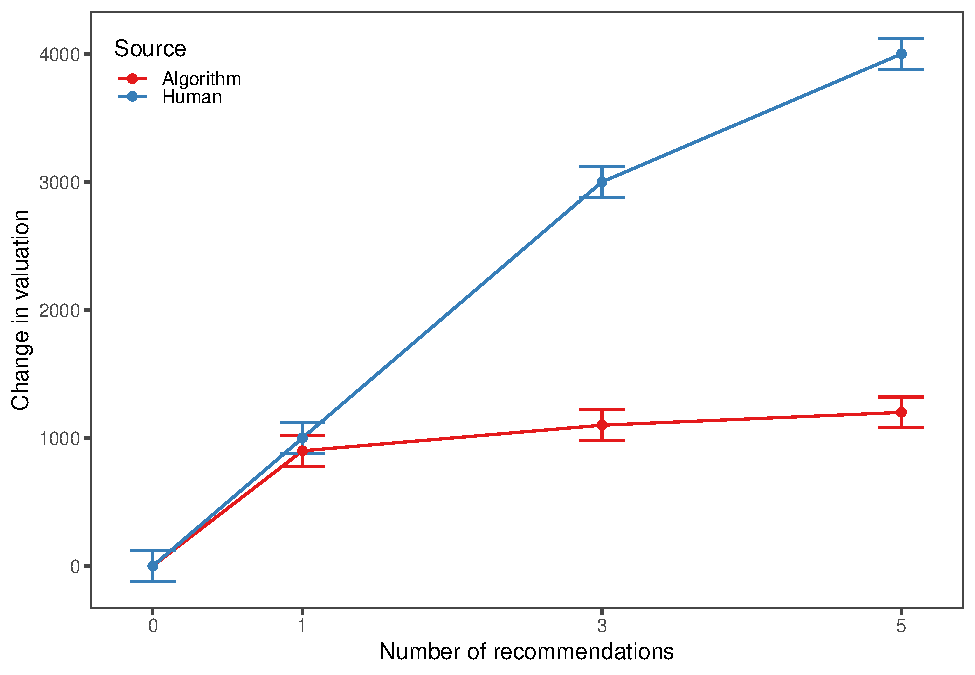
\includegraphics[width=.5\textwidth]{Test-Manuscript-in-R_files/figure-latex/hyp-1} 
\label{fig:hyp}
\end{figure}

\hypertarget{methods}{%
\section{Methods}\label{methods}}

\hypertarget{procedure}{%
\subsection{Procedure}\label{procedure}}

\begin{figure}
\caption{Procedure of the study. Top row shows the stimulus generating procedure, and bottom two rows show the practice and critical trials respectively.}\label{fig:procedure}
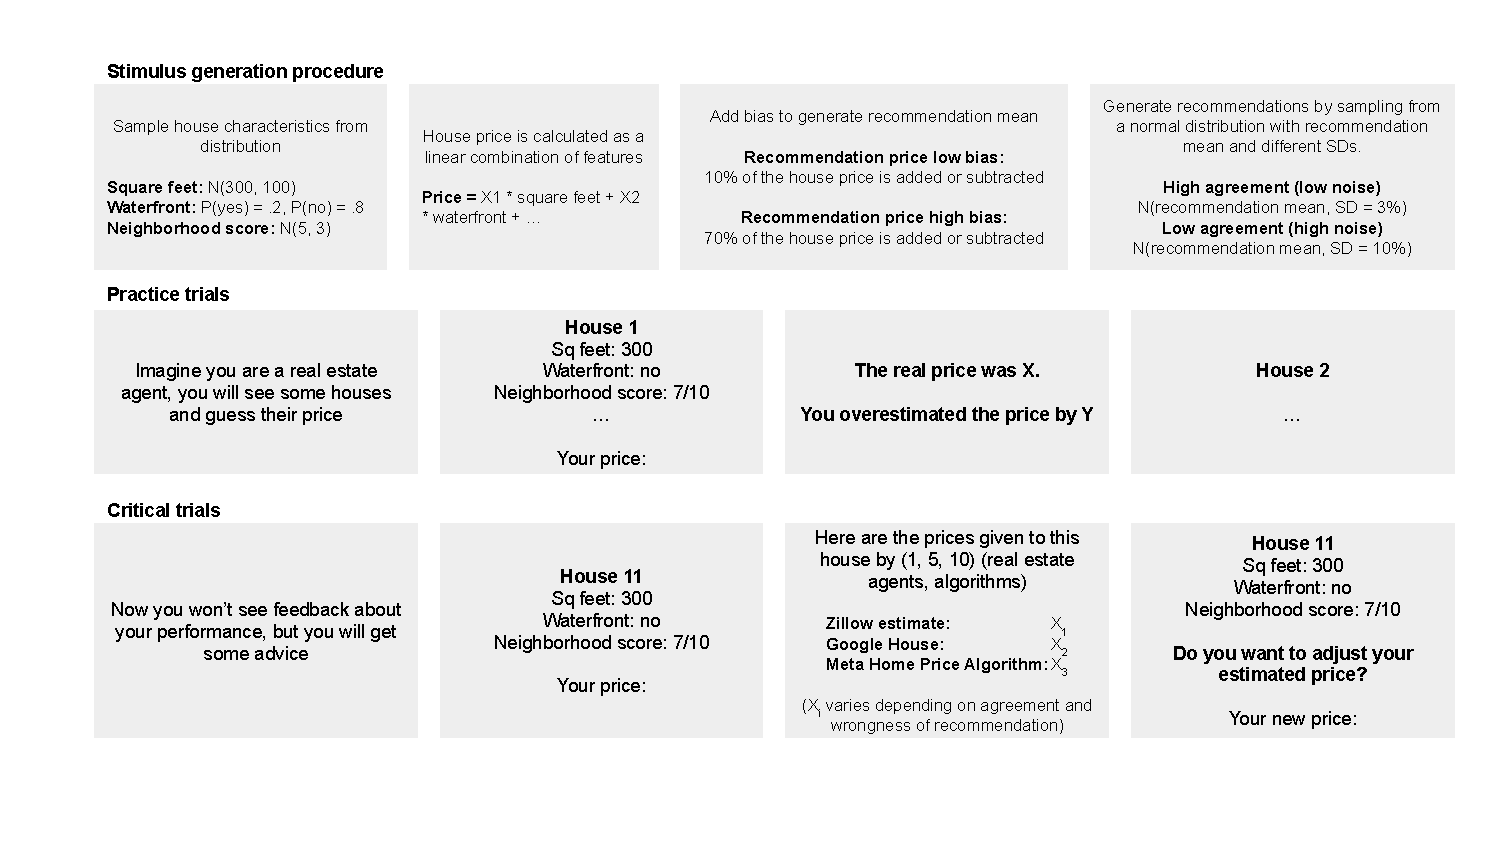
\includegraphics[width=\textwidth]{procedure} 
\end{figure}

Participants will being by reading an introduction to the task. They are going to see descriptions of houses, and will judge their price. All houses are located in the same city, and vary along dimensions of size, number of bedrooms and bathrooms, neighborhood characteristics, whether or not it is a waterfront home, among other house characteristics. House descriptions are generated by sampling from a distribution of characteristics, and their price is a linear combination of the features (See \textbf{Figure} \ref{fig:procedure} for a graphical representation of the stimuli generation procedure and the participant experience). In order to establish a common baseline for evaluating house prices, there will be a set of practice trials, where participants guess the house price, and receive feedback on the real price and how much they overestimated or underestimated the house price. Once participants achieve 4 trials where their accuracy is within 10\% of the real house price, they will begin the critical trials. This practice stage is designed to reduce noise in the ratings due to participants having different base rates for house prices, additionally, it will reduce the possibility that participants simply default to the recommendations because they feel like they don't know about house prices.

Before beginning the critical trials, participants will see a screen informing them that they will no longer receive feedback, but might get some advice, either from expert real estate agents from that city, or from house price prediction algorithms. Also, they will learn that performance in this stage will be rewarded, such that 10\% of the most accurate respondents will receive a bonus. Participants will see the house characteristics and guess its price. Then, they will see recommendations, and after that, decide whether or not they want to adjust their initial estimate.

After 48 randomized trials, participants will self-report their algorithm aversion in the financial domain, items on the perceived variance of algorithms, and a demographic questionnaire. Finally, participants will be debriefed about the house prices and recommendations being fake, and about their performance.

\hypertarget{participants}{%
\subsection{Participants}\label{participants}}

We will recruit 500 participants from Prolific, and each participant will complete 40 trials, for a total sample size of 20,000 trials. This will allow us to be powered for interaction effects, which require larger samples than what is usually considered (Simonsohn, 2014).

\hypertarget{materials}{%
\subsection{Materials}\label{materials}}

\hypertarget{self-report-measures}{%
\subsubsection{Self-report measures}\label{self-report-measures}}

\hypertarget{algorithm-appreciation-and-aversion.}{%
\paragraph{Algorithm appreciation and aversion.}\label{algorithm-appreciation-and-aversion.}}

We will 4 items out of the algorithm aversion scale (Melick, 2020) to ascertain baseline levels of trust and mistrust in algorithms, specifically in the financial domain. We hypothesize that people who score high in algorithm aversion will be less likely to conform to algorithms, but not to other people. Items are reproduced in the appendix.

\hypertarget{perceived-variance-in-algorithms.}{%
\paragraph{Perceived variance in algorithms.}\label{perceived-variance-in-algorithms.}}

If people react similarly to a single algorithmic recommendation as opposed to multiple, it may be because they believe that algorithms tend to be very similar among each other. If people think that algorithmic recommendations are highly correlated (or more correlated to each other than human judgment), then this could explain a potentially flatter relationship between number of recommendations and conformity.

Here are potential items for this scale: ``I think that most algorithms tend to give similar recommendations'', ``There is more variety in the judgments of experts than in those of algorithms'', ``All algorithms produce the same results''.

\hypertarget{manipulations}{%
\subsubsection{Manipulations}\label{manipulations}}

\hypertarget{source-of-opinions}{%
\paragraph{Source of opinions}\label{source-of-opinions}}

Across trials, participants will see house price recommendations that are provided by either a number of real estate agents, or a number of different algorithms.

\hypertarget{number-of-opinions}{%
\paragraph{Number of opinions}\label{number-of-opinions}}

Across trials, participants will receive recommendations from either 1, 3 or 5 different sources, either all algorithms, or all real-estate agents.

\hypertarget{agreement-between-opinions}{%
\paragraph{Agreement between opinions}\label{agreement-between-opinions}}

Across trial we will manipulate the level of agreement between the recommendations. In the low-agreement condition, the recommendations will be drawn from a normal distribution with 10\% of the house price as a standard deviation, whereas in the high-agreement condition, the standard deviation will be 3\% of the house price.

\hypertarget{bias-in-recommendations}{%
\paragraph{Bias in recommendations}\label{bias-in-recommendations}}

Recommendations will be either close to the actual price of the house (10\% higher or lower than real house price - low bias), or far from the actual house price (70\% higher or lower than the real house price - high bias).

\hypertarget{dependent-variable-change-in-house-price-rating}{%
\subsubsection{Dependent variable: Change in house price rating}\label{dependent-variable-change-in-house-price-rating}}

For each trial, the dependent variable will be the size of the adjustment from the original guess to the guess after seeing recommendations. A change of 0 means that participants did not change their response (indicating no conformity), positive scores indicate that the participant changed their response to be closer to the recommendations, and negative scores indicate that the participants score drifted away of recommendations (i.e., a reactance effect).

\hypertarget{analysis}{%
\subsection{Analysis}\label{analysis}}

Aside from the regular multilevel model to analyze the effect of each of the manipulations on the outcome, it would be interesting to analyze changes in conformity as the trials go on. I would hypothesize that conformity might increase as trials go by for people low in algorithm aversion, but might decrease as the trials go by for people high in algorithm aversion. People high in algorithm aversion might be more critical and attentive to the wrongness of the algorithmic predictions (Dietvorst et al., 2015) and might learn to ignore its recommendations. People low in algorithm aversion might get more and more comfortable with taking recommendations from the algorithm as the trials progress.

\hypertarget{discussion-potential-points}{%
\section{Discussion (Potential points)}\label{discussion-potential-points}}

How did conformity to human experts differ from conformity to algorithms?

\begin{itemize}
\item
  Human recommendations and algorithmic ones might differ in their levels of informational vs.~normative influence. Participants with higher levels of algorithm aversion could view algorithms as less informational.
\item
  It stands to reason that algorithms exert no normative influence, that is, participants are not worried about fitting in, or being liked by them. Advice from other humans might exert normative influence, but probably to a much lesser extent than in in-person lab studies of conformity.
\end{itemize}

Some ideas for limitations of the study:

\begin{itemize}
\item
  Participants in the study were non-experts. To limit the possibility that people might have different levels of experience with the housing market, we used an artificially created stimulus set, and participants practiced until they reached similar expert performance. However, non-experts are less prone to algorithm aversion (Logg et al., 2019), so rates of conformity produced by this study might be inflated compared to those that we would observe in the real world. Therefore, it would be ideal to replicate this study with expert decision makers (e.g., real estate agents, or admissions officers in a similar study for admissions decisions.)
\item
  In the real world, people might increasingly interact with both human and algorithmic advice concurrently. Take for example a situation where you are driving, and your friend suggests you take a different route to the one google maps recommends. This study did not shed light on how people react to algorithms and humans simultaneously. Thus, future research could test the effect of showing human and algorithmic advice concurrently.
\item
  In this study, we manipulated the number of sources, their level of wrongness (i.e., bias), and their agreement (i.e., noise) in a discrete manner. It could be that certain aspects of the functions that map the explanatory variables to the outcomes remain hidden in the \emph{in-between} levels of the explanatory variables. With our methodology, it would be possible to sample the space of explanatory variables continuously, by randomly sampling a number of sources, and the level of noise and bias for each trial.
\item
  This study lacked the powerful social situation of having other people present, and thus, the contribution of normative influence was minimized (But not necessarily eliminated, see Salganik et al. (2006)). Future research could have other people present, either in person or virtually (an interesting distinction yet to be explored, given that so much of communication is no longer face to face). In such a study, recommendations would be received from real estate agents, and a representative of the algorithm (e.g., someone who participated in its creation).
\item
  Another potential outcome of interest that we have not included in this study is the feeling of confidence in one's predictions. Perhaps algorithmic and human recommendations change the pricing of houses in similar ways, but the confidence associated with this judgments might be different.
\end{itemize}

\newpage

\hypertarget{references}{%
\section{References}\label{references}}

\hypertarget{refs}{}
\begin{CSLReferences}{1}{0}
\leavevmode\vadjust pre{\hypertarget{ref-amazons2018}{}}%
Amazon scraps secret AI recruiting tool that showed bias against women. (2018). \emph{Reuters}. \url{https://www.reuters.com/article/us-amazon-com-jobs-automation-insight-idUSKCN1MK08G}

\leavevmode\vadjust pre{\hypertarget{ref-apadict}{}}%
\emph{APA Dictionary of Psychology}. (n.d.). \url{https://dictionary.apa.org/}

\leavevmode\vadjust pre{\hypertarget{ref-asch1956}{}}%
Asch, S. E. (1956). Studies of independence and conformity: I. A minority of one against a unanimous majority. \emph{Psychological Monographs: General and Applied}, \emph{70}, 1--70. \url{https://doi.org/10.1037/h0093718}

\leavevmode\vadjust pre{\hypertarget{ref-asch1995}{}}%
Asch, S. E. (1995). Foundations of conformity and obedience. \emph{Psychological Dimensions of Organizational Behavior}, 267.

\leavevmode\vadjust pre{\hypertarget{ref-bernheim1994}{}}%
Bernheim, B. D. (1994). A Theory of Conformity. \emph{Journal of Political Economy}, \emph{102}(5), 841--877. \url{https://doi.org/10.1086/261957}

\leavevmode\vadjust pre{\hypertarget{ref-bond1996}{}}%
Bond, R., \& Smith, P. B. (1996). Culture and conformity: A meta-analysis of studies using asch's (1952b, 1956) line judgment task. \emph{Psychological Bulletin}, \emph{119}(1), 111--137.

\leavevmode\vadjust pre{\hypertarget{ref-brynjolfsson2017}{}}%
Brynjolfsson, E., \& Mitchell, T. (2017). What can machine learning do? Workforce implications. \emph{Science}, \emph{358}(6370), 1530--1534. \url{https://doi.org/10.1126/science.aap8062}

\leavevmode\vadjust pre{\hypertarget{ref-cialdini2004}{}}%
Cialdini, R. B., \& Goldstein, N. J. (2004). Social Influence: Compliance and Conformity. \emph{Annual Review of Psychology}, \emph{55}(1), 591--621. \url{https://doi.org/10.1146/annurev.psych.55.090902.142015}

\leavevmode\vadjust pre{\hypertarget{ref-dawes1979}{}}%
Dawes, R. M. (1979). The robust beauty of improper linear models in decision making. \emph{American Psychologist}, \emph{34}(7), 571--582. \url{https://doi.org/10.1037/0003-066X.34.7.571}

\leavevmode\vadjust pre{\hypertarget{ref-dawes1989}{}}%
Dawes, R. M., Faust, D., \& Meehl, P. E. (1989). Clinical versus actuarial judgment. \emph{Science}, \emph{243}(4899), 16681674.

\leavevmode\vadjust pre{\hypertarget{ref-deutsch1955}{}}%
Deutsch, M., \& Gerard, H. B. (1955). A study of normative and informational social influences upon individual judgment. \emph{The Journal of Abnormal and Social Psychology}, \emph{51}, 629--636. \url{https://doi.org/10.1037/h0046408}

\leavevmode\vadjust pre{\hypertarget{ref-dietvorst2015}{}}%
Dietvorst, B. J., Simmons, J. P., \& Massey, C. (2015). Algorithm Aversion: People Erroneously Avoid Algorithms After Seeing Them Err. \emph{Journal of Experimental Psychology: General}, \emph{144}(1), 114--126.

\leavevmode\vadjust pre{\hypertarget{ref-grove2000}{}}%
Grove, W. M., Zald, D. H., Lebow, B. S., Snitz, B. E., \& Nelson, C. (2000). Clinical versus mechanical prediction: A meta-analysis. \emph{Psychological Assessment}, \emph{12}, 19--30. \url{https://doi.org/10.1037/1040-3590.12.1.19}

\leavevmode\vadjust pre{\hypertarget{ref-kahneman2016a}{}}%
Kahneman, D., Rosenfield, A. M., Gandhi, L., \& Blaser, T. (2016). Noise. How to Overcome the High, Hidden Cost of Inconsistent Decision Making. \emph{Harvard Business Review}, 38--46.

\leavevmode\vadjust pre{\hypertarget{ref-kahneman2021}{}}%
Kahneman, D., Sibony, O., \& Sunstein, C. R. (2021). \emph{Noise: A flaw in human judgment}. Harper Collins.

\leavevmode\vadjust pre{\hypertarget{ref-kaufmann2021}{}}%
Kaufmann, E. (2021). Algorithm appreciation or aversion? Comparing in-service and pre-service teachers{'} acceptance of computerized expert models. \emph{Computers and Education: Artificial Intelligence}, \emph{2}, 100028. \url{https://doi.org/10.1016/j.caeai.2021.100028}

\leavevmode\vadjust pre{\hypertarget{ref-klucharev2009}{}}%
Klucharev, V., Hytönen, K., Rijpkema, M., Smidts, A., \& Fernández, G. (2009). Reinforcement Learning Signal Predicts Social Conformity. \emph{Neuron}, \emph{61}(1), 140--151. \url{https://doi.org/10.1016/j.neuron.2008.11.027}

\leavevmode\vadjust pre{\hypertarget{ref-liel2020}{}}%
Liel, Y., \& Zalmanson, L. (2020). \emph{What if an AI told you that 2 + 2 is 5? Conformity to algorithmic recommendations}.

\leavevmode\vadjust pre{\hypertarget{ref-logg2019}{}}%
Logg, J. M., Minson, J. A., \& Moore, D. A. (2019). Algorithm appreciation: People prefer algorithmic to human judgment. \emph{Organizational Behavior and Human Decision Processes}, \emph{151}, 90--103. \url{https://doi.org/10.1016/j.obhdp.2018.12.005}

\leavevmode\vadjust pre{\hypertarget{ref-melick2020}{}}%
Melick, S. R. (2020). \emph{Development and validation of a measure of algorithm aversion} {[}PhD thesis{]}. \url{https://www.proquest.com/docview/2405300583/abstract/4CA96334EBCA4475PQ/1}

\leavevmode\vadjust pre{\hypertarget{ref-riedl2019}{}}%
Riedl, M. O. (2019). Human{-}centered artificial intelligence and machine learning. \emph{Human Behavior and Emerging Technologies}, \emph{1}(1), 33--36. \url{https://doi.org/10.1002/hbe2.117}

\leavevmode\vadjust pre{\hypertarget{ref-salganik2006}{}}%
Salganik, M. J., Dodds, P. S., \& Watts, D. J. (2006). Experimental study of inequality and unpredictability in an artificial cultural market. \emph{Science}, \emph{311}(5762), 854--856. \url{https://doi.org/10.1126/science.1121066}

\leavevmode\vadjust pre{\hypertarget{ref-sawyer1966}{}}%
Sawyer, J. (1966). Measurement and prediction, clinical and statistical. \emph{Psychological Bulletin}, \emph{66}(3), 178.

\leavevmode\vadjust pre{\hypertarget{ref-shrestha2019}{}}%
Shrestha, Y. R., Ben-Menahem, S. M., \& Krogh, G. von. (2019). Organizational Decision-Making Structures in the Age of Artificial Intelligence. \emph{California Management Review}, \emph{61}(4), 66--83. \url{https://doi.org/10.1177/0008125619862257}

\leavevmode\vadjust pre{\hypertarget{ref-simonsohn2014}{}}%
Simonsohn, U. (2014). \emph{{[}17{]} no-way interactions}. \url{http://datacolada.org/17}

\leavevmode\vadjust pre{\hypertarget{ref-waters2013}{}}%
Waters, A., \& Miikkulainen, R. (2013). GRADE: Machine Learning Support for Graduate Admissions. \emph{Proceedings of the 25th Conference on Innovative Applications of Artificial Intelligence}, 8.

\leavevmode\vadjust pre{\hypertarget{ref-yeomans2019}{}}%
Yeomans, M., Shah, A., Mullainathan, S., \& Kleinberg, J. (2019). Making sense of recommendations. \emph{Journal of Behavioral Decision Making}, \emph{32}(4), 403--414. \url{https://doi.org/10.1002/bdm.2118}

\end{CSLReferences}

\newpage

\hypertarget{appendix}{%
\section{Appendix}\label{appendix}}

\hypertarget{algorithmic-aversion-and-appreciation-items---financial-domain.}{%
\subsection{Algorithmic aversion and appreciation items - Financial domain.}\label{algorithmic-aversion-and-appreciation-items---financial-domain.}}

Below are the items for the algorithm aversion scale in the financial domain (Melick, 2020).

\begin{itemize}
\item
  Financial advice that is index-based is more effective than financial advice that is based on the judgment of the advisor. (R)
\item
  It is more appropriate for financial advisors to make recommendations that are index based than to make recommendations that are based on their own judgment. (R)
\item
  It is more appropriate for financial lending institutions to make loan decisions based on a mathematical formula designed to predict probability of loan default than based on the judgment of the loan officer. (R)
\item
  Financial lending decisions that are based on the judgment of the loan officer are more effective than lending decisions that are based on the mathematical probability of loan default.
\end{itemize}


\end{document}
